Software Development Life Cycle (SDLC) is a way to systematically approach software development.
It provides a methodology to improve quality of the desired product and the general work progress. 
Depending on the customer or end users and how clear the project's requirements are different approaches are needed. 
Among the different SDLC methods are the most common ones the older traditional ''Waterfall model'' and the newer ''Iterative model''. \cite{SDLC-Toolsqa}


This chapter will first briefly present the ''waterfall model'' and the ''iterative model'', And during these the argument for choosing the ''iterative model''.
Hereafter, the chapter will contain a description of each iteration throughout the project.


\section{Waterfall model}
This section is based upon \cite{Waterfall-Toolsqa}.
%smid bogens titel ind 
%Anna: Astrid det er ikke en bog men en hjemmeside

The principle of the waterfall model is that the software development process is divided into separate phases, which makes it a sequential design process.
Here the output, in form of documentation, of one phase serves as the input for the next one which means that no phase will start without the previous one being complete.
This is often illustrated as a downward going flow, see \cref{fig:Waterfall}, which is also the reason for its name.

\begin{figure}[H]
	\centering
	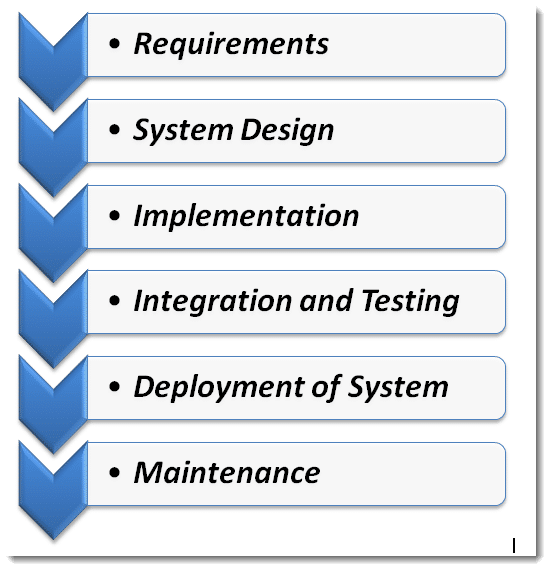
\includegraphics[width=0.4\textwidth]{billeder/WaterFall-Model.png}
	\caption{The Waterfall Model \cite{Waterfall-Toolsqa}.}\label{fig:Waterfall}
\end{figure}

\paragraph{The main benefits} of this model, is that it allows for departmentalization, which in theory makes it possible for separate teams to work at each phase without ever communicating with one another since only the documentation is necessary.
Another benefit of this system is how it is easy to manage since there are clear guidelines of what is needed before one phase is done and another can begin.

\paragraph{The main disadvantage} is on the other hand that because of this rigidity it becomes more difficult after every finished phase to go back and change things, when mistakes or misunderstandings of the concept has been made.
Therefore it is also not a beneficial model to use when there is a moderate to high risk that the requirements of the system changes.
%ville måske være bedre med en simpel textbf for at undgå ekstra mellemrum i pdfen
%Anna: Synes ikke selv det gør noget, kan god lide de to ting er skilt ad

Since the system developed in this project is done in cooperation with Ipsen, there is a moderate risk of the requirements changing.
This based on the risk of concept misunderstandings, since Ipsen is an expert in her field who has taken contact to software developers with no expertise in this field.
%ikke helt sikker på om jeg forstår this based delen af denne her sætning

\section{Iterative Model} \label{sec:iterativModel}
This section is based on \cite{InteractionDesign,Rod-Aalborg,Iterative-Toolsqa,Benyon}.
%vil igen argumentere for at der skal titel på
%Anna: det er ikke fordi det er normalt at gøre, normalt har man bare kilde referencen sat ind

The main principle of the iterative model is to divide the software development into a cycle of ''waterfalls'', it could also be seen as a form of ''multi-waterfalls'' model.
Instead of focusing on everything through every phase in the waterfall model, the development is done in pieces and at every iteration a little more is added to the product until it is finished.
The model usually has four basic activities, the formal names may change from the specific models but the idea is the same. 
Through each iteration the product and requirements are always being redetermined, redefined and further developed through the four main activities and in collaboration with the client or users, until the final solution is reached.
Different iteration models are simplified versions of reality and are not meant to be prescriptive, and depending on the project it is not always possible to go through all of the phases described in these models. 
Some explicit models will be presented in the \cref{sec:Iterative1,sec:Iterative2}.


\paragraph{The main benefits}
of working iteratively is the continuous talk with the client and users which yields the opportunity to determine and redetermine what their needs truly are rather than just what they believe them to be.
This ongoing communication also makes it easier for catching mistakes and faulty software since only a little part is added at each iteration.
It is easier as well to clarify misconceptions of the products requirements.
The repeated correspondence with the client and/or users is likewise the center of the user-centered approach, mentioned in \cref{sec:PACT}, which is of great importance when designing and developing an interactive system.
%måske få tydeligere frem at det er nemmere at opdage fejlene tidligere

\paragraph{The main disadvantage} of the iteration model is how adding functionality at every stage, may cause problems related to the system architecture since it had not been thought into the design to begin with.
This may in worst case scenario cause for the whole system to be redesigned at re-implemented.
Another disadvantage with this model is also one of it strong suits and allures, which is how it can become difficult to manage, and keep track of the development and when a iteration is done and a new one begin since it is ever changing.

\paragraph{Iterative model in design process:}
%Anna: Evt fjerne paragraph titlen ovenfor, er ikke sikker på om den i virkeligheden gør noget for det hele
As suggested in the disadvantages one of the allures of this iteration model is its ever changing quality and how it i more of a guideline which conforms to the different periods of the software development.
This suits the process of designing interaction system which is ''messy'' as the quote below from \citep[p.~156]{DesignerStance} illustrates.

''Remember, design is messy; designers try to understand the mess. They observe to how their products will be used; design is about users and use. They visualize, which is the act of deciding what it is.''

The Iteration proccess and the contentious communication with client and/or users is therefore a more natural way to develop human centered interaction systems.


\subsection{The process of designing interaction systems}\label{sec:Iterativedesign}
As mentioned in \cref{sec:iterativModel} there are usually four basic activities, which may be called differently in the different models, even though the basic idea is commonly the same.
In life cycle model in \cref{fig:LifeCycleModel} these activities are called;
\textit{establishing requirements, designing alternatives, prototyping,} and \textit{evaluating}. 

\begin{figure}[H]
	\centering
	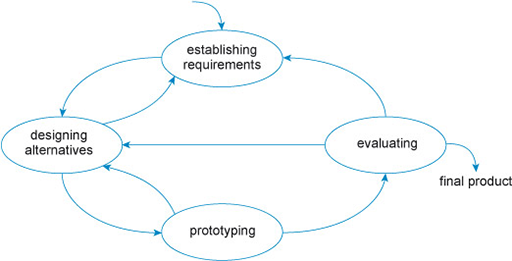
\includegraphics[width=0.75\textwidth]{billeder/lifecycle.png}
	\caption{Life cycle model \citep[p.~332]{InteractionDesign}}\label{fig:LifeCycleModel}
\end{figure}

To be able to design a system with the user’s needs and wants in mind it is imperative to know the target users and which activities the system needs to support. 
This is done through establishing requirements where information of the target users is gathered through data gathering and analysis. 
When the requirements are settled it is possible to design alternatives ideas that meet these suggested requirements. 
After the alternative design phase is completed a prototype can be developed. 
The purpose of the prototype is to evaluate with the users whether the criteria has been fulfilled and to present how the system could potentially turn out. 
Finally, when the prototype is complete it can be measured an evaluated. 
The evaluation phase determines whether or not the design is usable and/or acceptable and thereby if another design iteration is needed.

%Anna: tænker lidt vi enten bruger teksten ovenfor eller denne her nedenunder, synes det bliver meget dobbelt konfekt at bruge beggge.
According to Sharp, Rogers and Preece ''Most projects start with establishing requirements'' \citep[p.~333]{InteractionDesign}. It is from this first activity that it’s possible to go into the ‘designing alternatives’ activity from where a prototype in the ‘prototyping’ activity, can be developed which in turn can be evaluated by the users in the ‘evaluating’ activity. From this evaluation the designers can specify new or redefined requirements, or they can go directly to redesign or deem the project done. 

\subsubsection{Another take on the interaction design process}\label{sec:Iterativedesign2}
In \cref{fig:DEBModel} another model is shown, where it becomes more apparent how it might be difficult to define when an iteration ends and a new one begin since it is possible to start and any point and to move back and forth between the activities seen fit.

\begin{figure}[H]
	\centering
	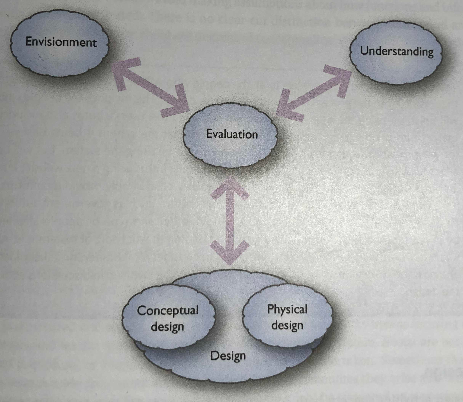
\includegraphics[width=0.5\textwidth]{billeder/DEBModel.png}
	\caption{Understanding, design, evaluation, envisionment \citep[p.~49]{Benyon}}\label{fig:DEBModel}
\end{figure}

The four basic activities of this model is instead of those shown above called; \textit{understanding, design, envisionment} and \textit{evaluation}.
though they correlate a lot with those before. 
'Understanding' is a broader term for 'establishing requirements' since it also covers topics such as understanding the context of the developed system and the technological landscape.
The 'envisionment' activity concerns itself with determining appropriate media in which to render design ideas.
While the 'design' activity is done through conceptual- and physical design as seen in \cref{fig:DEBModel}.
These two activities is together comparable to the 'designing alternatives' activity and 'prototyping' activity from \cref{fig:LifeCycleModel}.
'Evaluation' is the same in both models, it is the center of the process.

\subsection{OOA\&D iteration model}\label{sec:Iterative2}
In the OOA\&D method the four basic activities are; \textit{Problem-domain analysis, Application-domain analysis, Architectural design} and \textit{Component design}.
In between these activities  also lies programming and quality assurance.
The importance of each activity is relative in each iteration and the sequence changes from each development project.
Further down in this section two different models based on the OOA\&D method is presented.

%Anna: er det nødvendigt at skrive et afsnit om sammenligning af de fire aktiviteter?, da det i princippet er modeller til to forskellige ting tænker jeg ikke det er nødvendigt explicit at skrive ind her

In \cref{fig:SUModels} two different models based on the OOA\&D method is shown.
The first model, \cref{fig:SUModel1} is a model closer to the traditional waterfall model though it is still an iterative process modeled.
The second model, \cref{fig:SUModel2} is on the other hand closer to the stereotype of a iterative model where each phase is done or at least considered in every iteration.

\begin{figure}[H]
	\centering
	\begin{subfigure}[b]{0.48\textwidth}
		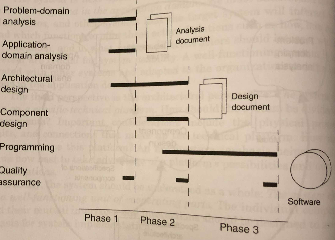
\includegraphics[width=\textwidth]{billeder/SUModel1.png}
		\caption{Traditional-top-down approach \citep[p.~16]{Rod-Aalborg}}
		\label{fig:SUModel1}
	\end{subfigure}
	\quad
	\begin{subfigure}[b]{0.48\textwidth}
		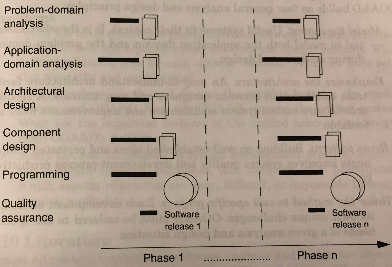
\includegraphics[width=\textwidth]{billeder/SUModel2.png}
		\caption{Use-case driven, arcitecture-centric approach \citep[p.~17]{Rod-Aalborg}}
		\label{fig:SUModel2}
	\end{subfigure}
	\caption{Model based on the OOA\&D method}\label{fig:SUModels}
\end{figure}


\subsection{Using iterative life cycle in the project}
Throughout the project it is intended to design a system iteratively with a specific user’s needs and wants integrated into the designs and tests. This is the basis of choosing to work with the iterative model to reflect over which activity is being used throughout the stages of the project.